\chapter{Unit Tests}
\section{10 Unit Tests}

\newcounter{rowcounter}
\newcommand\rownumber{\stepcounter{rowcounter}\arabic{rowcounter}}

\newcolumntype{b}{X}
\newcolumntype{s}{>{\hsize=.5\hsize}X}

\begin{table}[H]
	\centering
	\begin{tabularx}{\textwidth}{rs|b}
		& \textbf{Unit Test} & \textbf{Beschreibung} \\
		\midrule
		\rownumber & processTest:\newline HandleDartTest &
        Der Test \textit{processTest()} überprüft, ob die \textit{process()}-Methode der Klasse HandleDart die Eingabe des Benutzers korrekt verarbeitet und die erwarteten Dartpunkte zurückgibt. Der Test wird fünfmal wiederholt, um mehrere Eingaben zu simulieren und die Konsistenz der Ergebnisse zu überprüfen. \\
        \rownumber & playerDartStatusTest:\newline HandleDartTest &
        Der Test \textit{playerDartStatusTest()} überprüft, ob die Methode \textit{getDartStatus()} der Klasse \textit{HandleDart} den korrekten Dartstatus basierend auf dem aktuellen Punktestand und dem geworfenen Dart zurückgibt. Der Test verwendet verschiedene Dart-Eingaben und überprüft, ob der zurückgegebene Dartstatus den erwarteten Werten entspricht. \\
        \rownumber & getPlayerAverageOf\newline RoundTest:Player\newline AverageCalculatorTest &
        Der Test \textit{getPlayerAverageOfRoundTest()} überprüft, ob die Methode \textit{getPlayerAverageOfRound()} des \textit{PlayerAverageCalculator} die durchschnittlichen Punkte eines Spielers in einer Runde korrekt berechnet und zurückgibt. \\
        \rownumber & getPlayerAverageOf\newline LegTest:PlayerAverage\newline CalculatorTest &
        Der Test \textit{getPlayerAverageOfLegTest()} überprüft, ob die Methode \textit{getPlayerAverageOfLeg()} des \textit{PlayerAverageCalculator} die durchschnittlichen Punkte eines Spielers über alle Runden in einem \textit{Leg} korrekt berechnet und zurückgibt. \\
	\end{tabularx}
	\caption{Unit Tests 1-4}
	\label{tab:tests}
\end{table}

\begin{table}[H]
	\centering
	\begin{tabularx}{\textwidth}{rs|b}
		& \textbf{Unit Test} & \textbf{Beschreibung} \\
		\midrule
        \rownumber & getPlayersAveragesOf\newline LegTest:Player\newline AverageCalculatorTest &
        Der Test \textit{getPlayersAveragesOfLegTest()} überprüft, ob die Methode \textit{getPlayersAveragesOfLeg()} des \textit{PlayerAverageCalculator} die durchschnittlichen Punkte aller Spieler in einem \textit{Leg} als \textit{Map} zurückgibt und ob die berechneten Durchschnittswerte den erwarteten Werten entsprechen. \\
        \rownumber & getPlayerCheckoutQuote\newline OfLegTest:PlayerCheck-outQuoteCalculatorTest &
        Der Test \textit{getPlayerCheckoutQuoteOfLegTest()} überprüft, ob die Methode \textit{getPlayerCheckoutQuoteOfLeg()} des \textit{PlayerCheckoutQuoteCalculator} den Checkout-Anteil (Prozentsatz des erfolgreichen Checkouts im Vergleich zu den möglichen Checkouts) eines bestimmten Spielers in einem Leg korrekt berechnet und zurückgibt. Der Test überprüft, ob der berechnete Anteil mit dem erwarteten Wert übereinstimmt. \\
        \rownumber & getPlayersCheckoutQuote\newline OfLegTest:PlayerCheck-outQuoteCalculatorTest &
        Der Test \textit{getPlayersCheckoutQuoteOfLegTest()} prüft, ob die Methode \textit{getPlayersCheckoutQuoteOfLeg()} des \textit{PlayerCheckoutQuoteCalculator} eine Map zurückgibt, die die Checkout-Prozentsätze aller Spieler in einem Leg enthält. Der Test überprüft, ob die berechneten Anteile für jeden Spieler mit den erwarteten Werten übereinstimmen. \\
        \rownumber & getUserInputTest:\newline UserCommunication\newline ServiceTest &
        Der Test \textit{getUserInputTest()} überprüft, ob die Methode \textit{getUserInput()} des \textit{UserCommunicationService} die Benutzereingabe korrekt abruft und als \textit{UserInput}-Objekt zurückgibt. Dabei wird eine vordefinierte Zeichenkette als simulierter Benutzereingabe verwendet, und der Test vergleicht, ob die Rückgabewerte der Methode für jede Zeile der simulierten Eingabe den erwarteten Werten entsprechen. \\
	\end{tabularx}
	\caption{Unit Tests 5-8}
	\label{tab:tests}
\end{table}

\begin{table}[H]
	\centering
	\begin{tabularx}{\textwidth}{rs|b}
		& \textbf{Unit Test} & \textbf{Beschreibung} \\
		\midrule
        \rownumber & isValidDartValid\newline CaseTest:UserInputTest &
        Der Test \textit{isValidDartValidCaseTest()} überprüft, ob die Methode \textit{isValidDart()} der Klasse \textit{UserInput} den Wert \textit{true} zurückgibt, wenn die Eingabe ein gültiger Dartwert ist. In diesem Fall wird überprüft, ob \textit{SBull} als gültiger Dartwert erkannt wird. \\
        \rownumber & prepareUserDartInput\newline SBullTest:UserInputTest &
        Der Test \textit{prepareUserDartInputSBullTest()} überprüft, ob die Methode \textit{prepareUserDartInput()} der Klasse \textit{UserInput} die Benutzereingabe \textit{25} korrekt in den Dartwert \textit{SBull} umwandelt und als \textit{UserInput}-Objekt zurückgibt. Dabei wird überprüft, ob das umgewandelte Objekt den erwarteten Wert \textit{SBull} hat. \\
	\end{tabularx}
	\caption{Unit Tests 9-10}
	\label{tab:tests}
\end{table}
\section{ATRIP: Automatic}
\begin{enumerate}
    \item Einfache Ausführung: Die Unit Tests werden ausgeführt und die Ergebnisse werden in der Konsole ausgegeben.
    \item Automatisches Ablaufen: Durch die Verwendung eines global zugänglichen Scanners, kann die Systemeingabe vom Test gesetzt werden und durch den öffentlichen Scanner immer wieder weitere Zeilen aufgerunfen werden.
    \item Selbstüberprüfung: Die Unit Tests liefern durch Asserts, wie AssertEquals oder AssertTrue immer nur das Ergebnis Bestanden / Nicht Bestanden.
\end{enumerate}\newpage
\section{ATRIP: Thorough}
\textbf{Positiv Beispiel:}\\
\begin{figure}[ht]
    \centering
    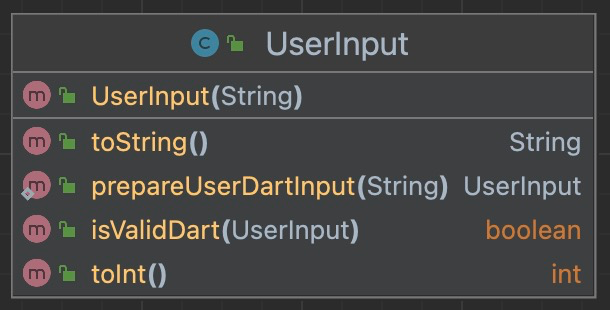
\includegraphics[width=0.8\textwidth]{Bilder/UserInputUML.png}
    \caption{UserInput UML}
    \label{fig:userinput-uml}
\end{figure}
In dieser Klasse wurden nur die Methoden \textit{isValidDart} und \textit{prepareUserDartInput} aktiv getestet. Es wurde sich dafür entschieden, da nur diese kritische und eventuell fehlerbehaftete Teile des Systems sind. Die Methoden \textit{toInt} und \textit{toString} sind hingegen kleine Hilfsmethoden, deren falsche Implementierung einen ebenso negativen Effekt auf die Anwendung hätte, jedoch sind diese Vergleichbar mit einer \textit{Getter} -und \textit{Setter}-Methode und sind somit trivial.\\
\lstinputlisting[
	label=code:userinputtest,    % Label; genutzt für Referenzen auf dieses Code-Beispiel
	caption=UserInputTest isValidDart-Methode,
	captionpos=b,               % Position, an der die Caption angezeigt wird t(op) oder b(ottom)
	style=EigenerJavaStyle,     % Eigener Style der vor dem Dokument festgelegt wurde
	firstline=1
]{Quellcode/UserInputTest.java}
Dieser Code Ausschnitt zeigt zwei Test-Methoden für die \textit{isValidDart}-Mathode. Dadurch werden beide Fälle der Methode abgedeckt: Ein gültiger Dart und ein ungültiger Dart.\\
\begin{figure}[ht]
    \centering
    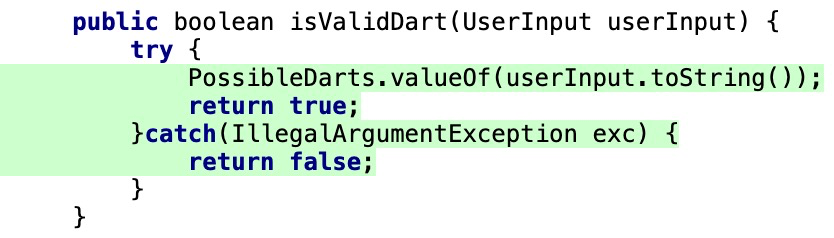
\includegraphics[width=0.8\textwidth]{Bilder/thoroughexample.png}
    \caption{vollständig abgedeckte Methode \textit{isValidDart}}
    \label{fig:isValidDart-Coverage-Code}
\end{figure}\\
Wie auf diesem Bild zu sehen ist, wurde die Methode \textit{isValidDart} vollständig abgedeckt. Dies bedeutet, dass alle möglichen Pfade der Methode durchlaufen wurden.\\\\
\textbf{Negativ Beispiel:}\\
\begin{figure}[ht]
    \centering
    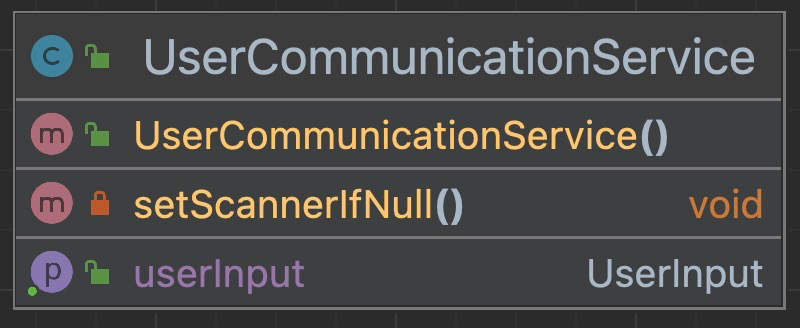
\includegraphics[width=0.8\textwidth]{Bilder/UserCommunicationServiceUML.png}
    \caption{UserCommunicationService UML}
    \label{fig:usercommunicationservice-uml}
\end{figure}
\lstinputlisting[
	label=code:usercommunicationservicetest,    % Label; genutzt für Referenzen auf dieses Code-Beispiel
	caption=UserCommunicationServiceTest Klasse,
	captionpos=b,               % Position, an der die Caption angezeigt wird t(op) oder b(ottom)
	style=EigenerJavaStyle,     % Eigener Style der vor dem Dokument festgelegt wurde
	firstline=1
]{Quellcode/UserCommunicationServiceTest.java}\newpage
\begin{figure}[ht]
    \centering
    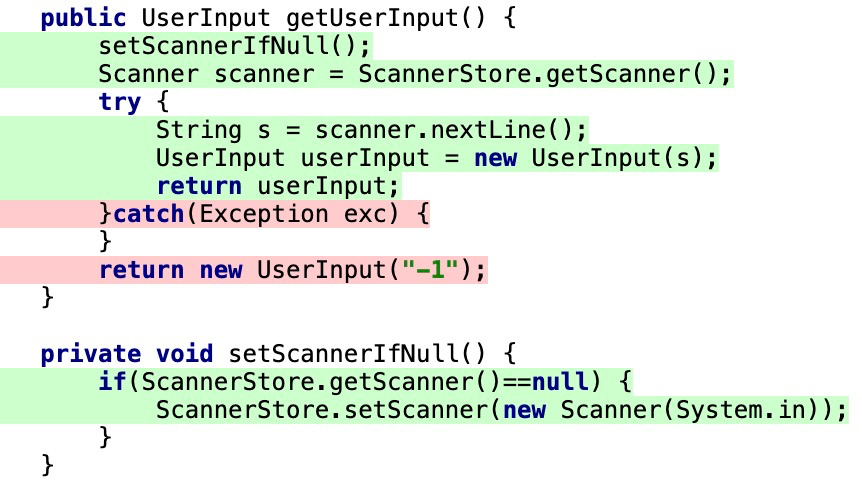
\includegraphics[width=0.8\textwidth]{Bilder/UserCommunicationService-Thorough.png}
    \caption{UserCommunicationService abgedeckter Code}
    \label{fig:usercommunicationservice-abgedeckter-code}
\end{figure}
Dieses Beispiel bezieht sich auf die Klasse \textit{UserCommunicationService}, welche für die Benutzerinteraktion verantwortlich ist. Sie verfügt über eine Methode zur Erfassung der Benutzereingaben und zur Umwandlung dieser in ein \textit{UserInput}-Objekt. Obwohl der Code innerhalb des \textit{try}-Blocks normalerweise keine Probleme verursachen sollte, muss dennoch ein Verhalten der Anwendung definiert sein, das im Fehlerfall ausgeführt werden kann. Sollte es unerwartet zu einem Fehler kommen und dieses Verhalten ausgeführt werden, würde der Test fehlschlagen und das Verhalten der Anwendung wäre unvorhersehbar. Daher erfüllt dieser Test nicht das Kriterium Thorough aus dem ATRIP-Prinzip, da er einen wesentlichen Teil des Systems, auf dem die Anwendung basiert, nicht abdeckt.
\section{ATRIP: Professional}
\textbf{Positiv Beispiel:}\\
\lstinputlisting[
	label=code:create-leg,    % Label; genutzt für Referenzen auf dieses Code-Beispiel
	caption=\textit{createLeg}-Funktion der Unit Test Klasse \textit{PlayerAverageCalculatorTest},
	captionpos=b,               % Position, an der die Caption angezeigt wird t(op) oder b(ottom)
	style=EigenerJavaStyle,     % Eigener Style der vor dem Dokument festgelegt wurde
	firstline=1
]{Quellcode/createLeg_PlayerAverageCalculatorTest.java}
In der Unit Test Klasse \textit{PlayerAverageCalculatorTest} wurde die Methode \textit{createLeg} implementiert. Diese Methode wird in der \textit{setup()}-Methode aufgerufen. Durch die Auslagerung des Codes in diese Methode, kann der Code für zukünftige Tests wiederverwendet werden.\\
\lstinputlisting[
	label=code:playerListe,    % Label; genutzt für Referenzen auf dieses Code-Beispiel
	caption=\textit{players}-Liste der Unit Test Klasse \textit{PlayerAverageCalculatorTest},
	captionpos=b,               % Position, an der die Caption angezeigt wird t(op) oder b(ottom)
	style=EigenerJavaStyle,     % Eigener Style der vor dem Dokument festgelegt wurde
	firstline=1
]{Quellcode/playersListe_PlayerAverageCalculatorTest.java}
Zuvor wurden 2 \textit{Player}-Objekte initialisiert, doch um die Erweiterbarkeit der Klasse zu verbessern wurden diese 2 Objekte in eine Liste aus Spielern gespeichert. Dadurch kann in Zukunft die Anzahl der Spieler erhöht werden, ohne dass der Code der Unit Test Klasse angepasst werden muss.\newpage
\textbf{Negativ Beispiel:}\\
\begin{figure}[ht]
    \centering
    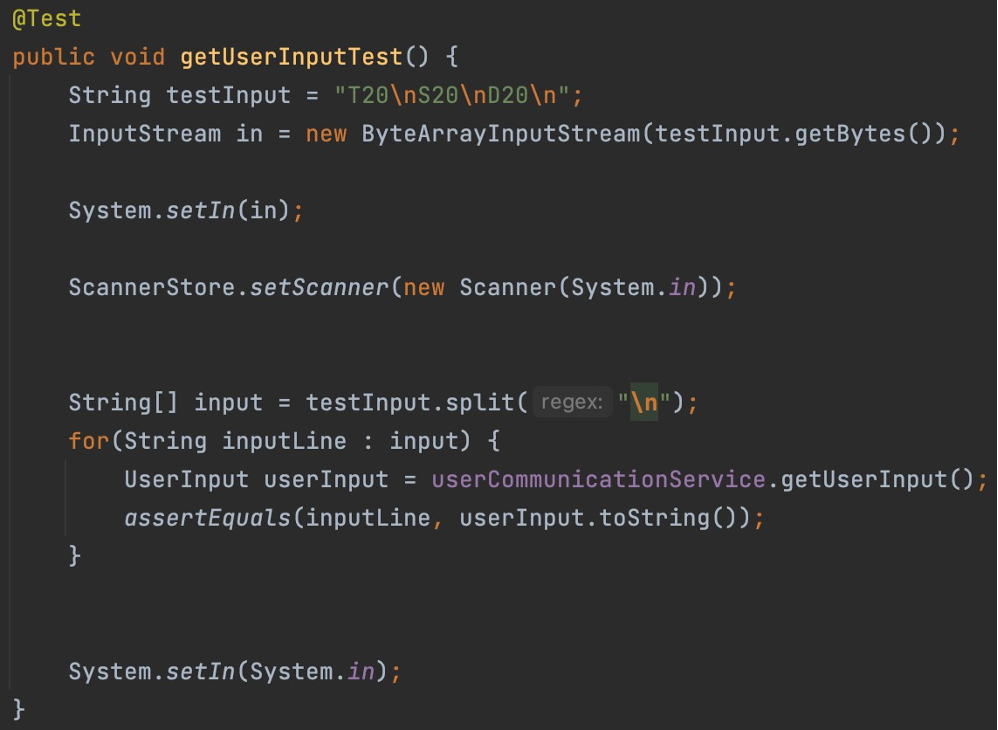
\includegraphics[width=0.8\textwidth]{Bilder/getUserInputTestCode.png}
    \caption{\textit{getUserInputTest}-Methode der Unit Test Klasse \textit{UserCommunicationServiceTest}}
    \label{fig:getUserInputTest-function}
\end{figure}\\
Als Negativ Beispiel könnte die Methode \textit{getUserInputTest} der Unit Test Klasse \textit{UserCommunicationServiceTest} dienen. Diese Methode ist für einen Entwickler, der nicht an der Entwicklung der Anwendung beteiligt war, nicht verständlich. Dies liegt daran, dass alle Operationen in einer Klasse geschehen. Durch die Einführung von Methoden, die den Code in kleinere Teile aufteilen, könnte die Lesbarkeit des Codes und die Wiederverwendbarkeit von Code-Teilen verbessert werden.\\
\section{Code Coverage}
Im Rahmen des Testens der Applikation wurde eine gezielte Vorgehensweise bei der Erstellung der Unit-Tests verfolgt. Es wurde dabei berücksichtigt, dass nicht für jede Klasse Tests notwendig sind, sondern ein Fokus auf jene gelegt wurde, die für den Verlauf der Anwendung als relevant erachtet wurden.

Die Konzentration lag insbesondere auf Klassen oder Methoden, die durch ihre Komplexität oder Wichtigkeit in der Anwendung hervorstechen. Ein Beispiel hierfür ist die Berechnung des Player-Average, welche eine komplexere Berechnung in vielen Teilen darstellt und daher explizit getestet wurde.

Aus diesem Grund wurden ausschließlich Tests für die Application-Layer entwickelt, da sie eine entscheidende Rolle für den Verlauf der Anwendung spielt. Die in dieser Schicht enthaltenen Klassen und Methoden haben direkte Auswirkungen auf den Anwendungsverlauf, weshalb ihre korrekte Funktion von großer Bedeutung ist.

Trotz alleinigen Testens der Application-Layer, blieb die Domain-Layer nicht unbeachtet. Viele der Klassen und Methoden dieser Schicht wurden passiv durch die Unit-Tests in der Application-Layer abgedeckt. Dies hat dazu geführt, dass die Domain-Layer eine Line-Coverage von knapp 50\% erreicht hat.

Zusammengefasst lässt sich sagen, dass durch diese Vorgehensweise eine gute und effiziente Testabdeckung erreicht wurde, die einen guten Überblick über den Zustand und die Qualität der Anwendung gibt.\newpage
\begin{figure}[ht]
    \centering
    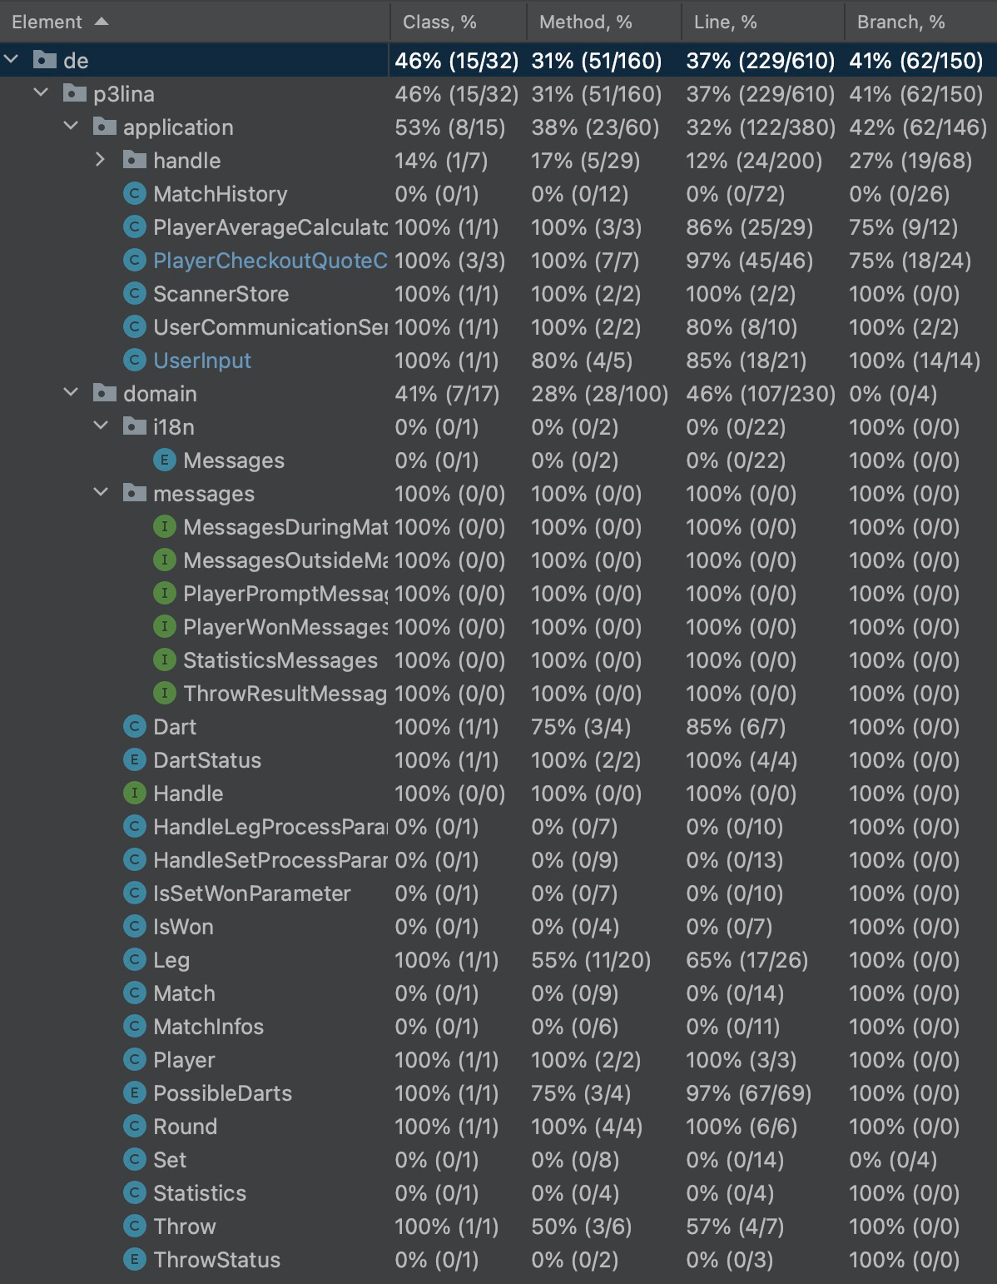
\includegraphics[width=0.7\textwidth]{Bilder/testCoverage.png}
    \caption{Überblick über die Test Coverage}
    \label{fig:test-coverage}
\end{figure}
\autoref{fig:test-coverage} gibt einen Überblick über die Abdeckung der implementierten Tests.\newpage
\section{Fakes und Mocks}
\begin{figure}[ht]
    \centering
    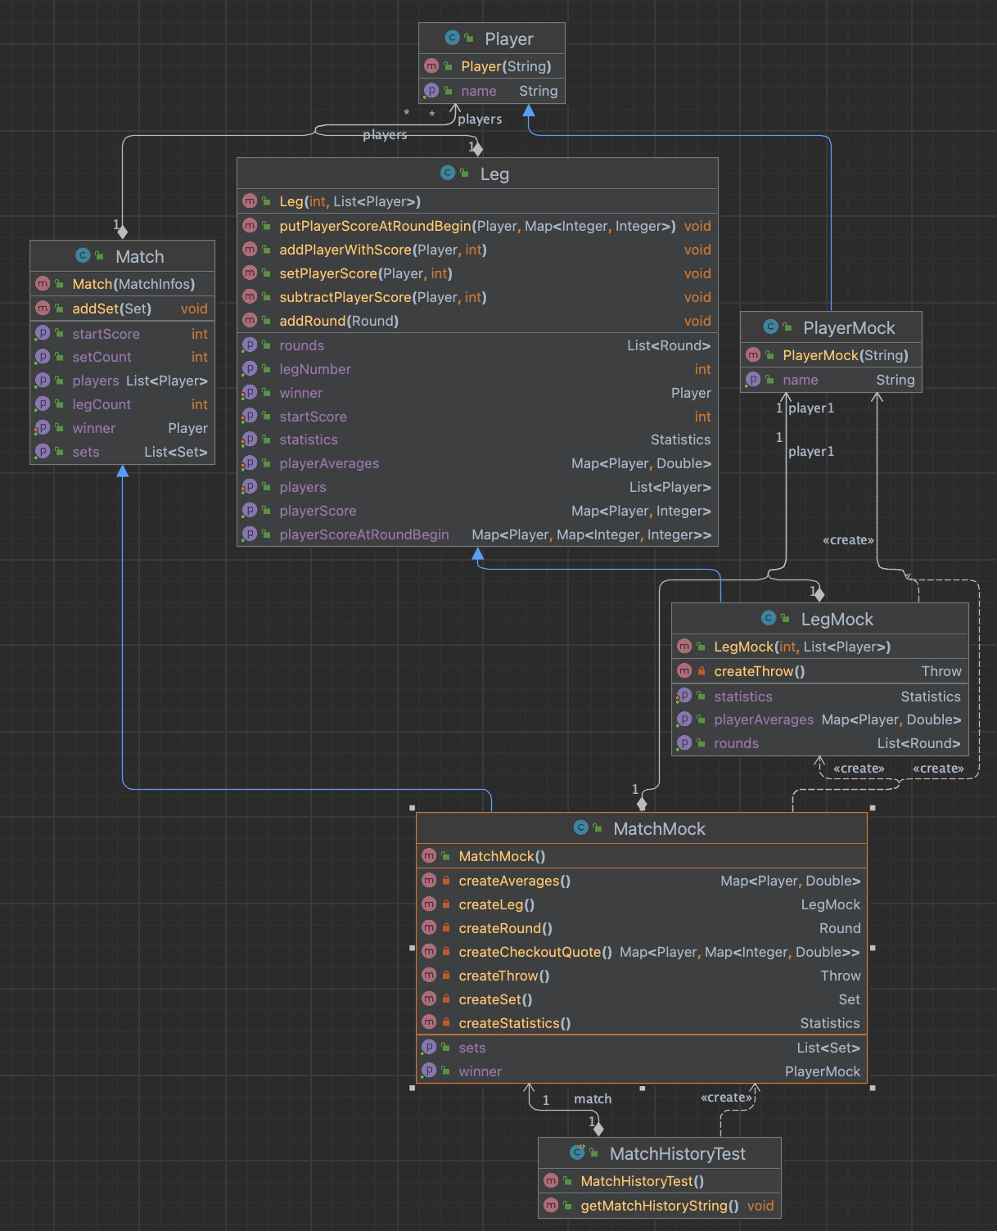
\includegraphics[width=0.8\textwidth]{Bilder/MockOverview.png}
    \caption{Übersicht der Mock-Klassen}
    \label{fig:mock}
\end{figure}
In der Unit Test Klasse \textit{MatchHistoryTest} werden zwei Fake- bzw. Mock-Objekte verwendet, um die Funktionalität der \textit{getMatchHistoryString} Methode in der MatchHistory Klasse zu testen. Die zwei Mock-Objekte, \textit{PlayerMock} und \textit{MatchMock}, simulieren das Verhalten realer Objekte innerhalb eines isolierten Testumfelds.

\textit{PlayerMock} dient dazu, das Verhalten eines \textit{Player}-Objekts zu imitieren, insbesondere im Hinblick auf die Rückgabe eines spezifischen Spielernamens. Auf der anderen Seite stellt \textit{MatchMock} ein komplexeres Szenario dar, in dem ein vollständiges Dartspiel mit Sets, Legs, Runden und Würfen simuliert wird.

Der Einsatz dieser Mock-Objekte ist wichtig, da es das Testen der getMatchHistoryString Methode ermöglicht, ohne von den tatsächlichen Implementierungen der Player und Match Klassen abhängig zu sein. Dies ist besonders nützlich, da die realen Klassen, vor allem die Match-Klasse, komplex sind.

Diese Mock-Objekte erlauben das Erstellen von vorhersehbaren Testszenarien. In diesem Fall kann garantiert werden, dass der \textit{getMatchHistoryString} Methode immer das gleiche Match mit den gleichen Spielern übergeben wird, wodurch der erwartete Ausgabestring konstant bleibt.